\documentclass[12pt]{article}
\usepackage[utf8]{inputenc,graphicx, booktabs, array} % Required for inserting images
\usepackage[paperheight=10.75in,paperwidth=8.25in,margin=1in,heightrounde]{geometry}
\usepackage[british]{babel}
\usepackage{indentfirst, amsmath}
\linespread{1.5}
\title{Prírodovedecká fakulta Univerzity Karlovej \\ 
\Large Katedra aplikovanej geoinformatiky a kartografie}
\date{}

\begin{document}

\maketitle
\vspace*{-2cm}
\begin{center}

\includegraphics[scale=0.4]{latex/image/logo.png} 
\end{center}

\begin{center}
\textbf {Algoritmy počítačovej kartografie}\\
\textit{Zadanie č. 2: Generalizovanie budov}\\
\vspace*{2cm}

\author {Bc. Filip Kradijan Seider\\Bc. Peter Dúbrava} \\
\date {2023/2024}
\\\LaTeX\
\end{center}
\thispagestyle{empty}
\newpage
\section*{Zadanie}\\
\noindent Vstup: množina budov $B = \{B_i\}_{i=1}^n$, budova $B_i = \{P_{i,j}\}_{j=1}^m$.}  \\
Výstup: $G(B_i)$.\\
\text{\par Zo súboru vyberiete vstupné údaje, ktoré predstavujú lomové body budov, a zovšeobecníte budovy na úroveň podrobnosti LOD0. Na tieto účely použite vhodný súbor údajov, napr. ZABAGED, otestujte nad tromi súbormi údajov (historické centrum mesta, intravilán - okolie, intravilán - izolovaná zástavba).\\  Pre každú budovu určte jej hlavné smery metódami:} 
\begin{itemize}
    \item Minimum Area Enclosing Rectangle,
    \item PCA.
\end{itemize}
\text
\par{Pri prvej metóde použite jeden z algoritmov na konštrukciu konvexného trupu. Pri generalizácii budovy na úroveň LOD0 nahraďte budovu obdĺžnikom orientovaným v oboch hlavných smeroch so stredom v strede budovy, jeho plocha bude rovnaká ako plocha budovy.Výsledky generalizácie vhodne vizualizujte. \par Otestujte a porovnajte účinnosť oboch metód pomocou hodnotových kritérií. Pokúste sa rozhodnúť, pre ktoré tvary budov poskytujú metódy nevhodné výsledky a pre ktoré poskytujú vhodnú aproximáciu.\\} 


\begin{table}[htbp]
    \centering  
    \footnotesize
    \begin{tabular}{m{12cm}c}
        \toprule 
        \bfseries Úloha & \bfseries Hodnotenie \\ 
        \midrule 
        Generalizovanie budov matódami Minimum Area Enclosing Rectangle a PCA& 15b \\
        Generalizovanie budov metódou Longest Edge& +5b \\
        Generalizovanie budov metódou Wall Average& +8b \\
        Generalizovanie budov metódou Weight Bisector& +10b \\
        Implementovanie ďalších metód tvorby konvexnej obálky& +5b \\
        Ošetrenie singulárnych prípadov pri generovaní konvexnej obálky & +2b \\
        \bottomrule 
        \bfseries Spolu & \bfseries 45b
    \end{tabular}
\end{table}

\newpage

\section*{Problematika}
Geoinformatika je vedná, ale aj technická disciplína, ktorá sa zaoberá používaním metód a vývojom aplikácií na riešenie geografických problémov. Hlavný dôraz je pritom kladený na určovanie polohy objektov v priestore a ich následné spracovanie v digitálnej podobe. Za týmto účlom je potrebné  preskúmať a zaznnamenať celý svet. To však prakticky nie je možné z viacerých dôvodov, pričom sa hlavne jedná o veľký nárok na výpočtovú techniku, či úložný priestor. Podobne ako napríklad v analógovej kartografii, kedy v závyslosti od mierky, či jej obsahu, dochádza kvôli výpovednej hodnote  a čitateľnosti mapy  ku zjednodušovaniu tvaru objektov. Tomuto procesu sa nevyhneme ani v súčastnej dobe.

Generalizácia je dôležitým nástrojom v geoinformatike a kartografii, ktorý umožňuje efektívne spravovať, analyzovať a vizualizovať geografické údaje v rôznych kontextoch a aplikáciách. Pri budovách sa stretávame so skratkou LOD (level of details) definujúcou množstvo detailov reálnych objektov sveta, od hrubých obrysov až po sofistikované 3D modely (3DBuildings, 2020). \par Prvá úroveň je LOD0 a predstavuje 2,5D digitálny model povrchu. LOD1 je kvádrový model budovy bez strešných štruktúr a bez textúry. Obohatením o strechu získavame LOD2. LOD3 je vytvorený pridaním architektonických informácií s detailami múrov a zobrazením menších štruktúr na strechách.Posledný je model LOD4, ktorý obsahuje všetky informácie o budove, vrátane jej interiéru. Spomína sa už aj LOD5, ktorá ale opisuje napríklad vlastnosti materiálov, stavebné metódy a požiadavky na údržbu (Trhan, 2017).
\begin{figure} [h]
    \centering
    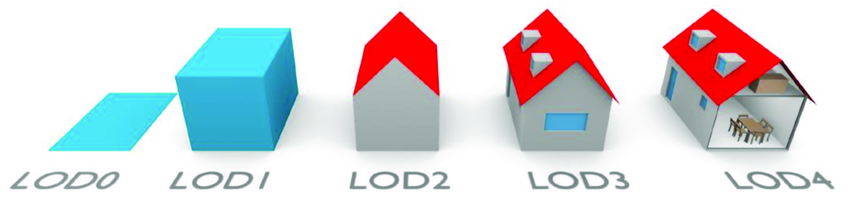
\includegraphics[width=0.7\linewidth]{latex/image/lod.png}
    \caption{Znázornenie detailu jednotlivých úrovní}
    \label{fig:enter-label}
\end{figure}
\subsection*{Konvexná obálka}
Konvexná obálka (\mathcal{H}), po anglicky convex hull, je jedna z narozšírenejších štruktúr v počítačovej geometrii, ktorá má svoje využitie samostatn, ale aj ako nástroj na vytváranie ďalších štruktúr (Rourke, 2005). Už podľa slovíčka konvexný usudzijeme, že spojnice medzi ľubovoľnými dvoma bodmi leží úplne vnútri tejto množiny. Konvexná obálka (\( H \)) môže existovať v ľubovoľnom priestore \( \mathbb{R}^d \), ktorý má \( d \) rozmerov, kde \( d \) je prirodzené číslo. Avšak v tomto prípade budeme špecificky skúmať konkrétnu variantu v dvojrozmernom priestore, \( \mathbb{R}^2 \), teda v rovine (\( p_i = [x_i, y_i] \)). Táto konkrétna verzia konvexnej obálky sa obmedzuje na prácu v rovine, kde sú objekty reprezentované dvojrozmernými súradnicami. Ďalej je definovaná aj ako konečná množina \( S \) predstavujúca :
\begin{itemize}
    \item konvexný mnohoúhelník \( P \) s najmenšou plochou,
    \item priesečnicu všetkých polrovín obsahujúcich \( P \),
    \item spojnicu všetkých trojuholníkov, ktorých vrcholy tvoria body \( P \).\\
\end{itemize} 
\par Využíva sa napríklad pri analýze tvaru objektu, vytváraní najmenšieho možného obdĺžnika obklopujúceho nejaký objekt (detekcia tvaru a otočenia objektu), detekcii kolízií (pohyb robotov), či analýze zhlukov (Bayer, 2024).
\par Jej zostrojenie je možné hneď viacerými spôsobmi, pričom nie všetky metódy je možné rozšíriť do vyššej dimenzie. Metódy majú rôzne výhody a nevýhody v závislosti na rozložení a množstve bodov, ale aj ďalších faktoroch. Napríklad rýchlosť tvorby konvexnej obálky s metódou Jarvis Scan je rýchlejší pri menej komplexných dátach, zatiaľ čo Grahamov Scan, je  efektívnejší pre veľké datasety. Práve na tieto dve metódy sa pozrieme bližšie a porovnáme si ich (Violentyev, 2020).

\begin{figure}[h]
    \centering
    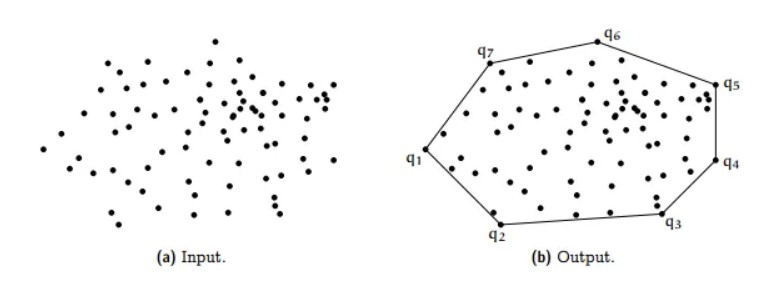
\includegraphics[width=0.8\linewidth]{latex/image/hull.jpg}
    \caption{Tvorba konvexnej obálky}
    \label{fig:enter-label}
\end{figure} \\
\newpage
\subsubsection*{Graham Scan}
Algoritmus Graham Scan podstatne zmenil výpočtovú geometriu poskytnutím riešenia problému konvexného obalu s vynikajúcou časovou zložitosťou \(O(n log n)\), kde n je počet vstupných bodov. Začína výberom dolného bodu (pivot \(q\)), typicky toho s najnižšou Y súradnicou, pretože je zaručené, že bude súčasťou konvexného obalu. Môže ale nastať situácia, že existuje viacero bodov s rovnakou súradnicou Y, preto je potrebné hľadieť aj na minimálnu hodnotu X, $$\min\limits_{\forall p_i \in S} = (x_i,y_i).$$
\par Potom zostávajúce body usporiada podľa ich uhlov vzhľadom na tento dolný bod a horizontálnu os. Ďalej prechádza týmito usporiadanými bodmi v protismeru hodinových ručičiek. Každý bod je pridaný do zásobníka, ak spĺňa podmienku ľavotočivosti s predchádzajúcimi dvoma bodmi v zásobníku. Pokiaľ to nespĺňa, tak sa vrátime o krok späť a daný bod už nebudeme používať. Tento proces efektívne konštruuje konvexný obal (Rourke, 1997; Violentyev 2020 ).  \\
\begin{equation}\nonumber
    p_j=
    \begin{cases}
    \notin \mathcal{H}, \quad p_{i+1} \in (p_i, p_{j+1}), \\
    ? \in \mathcal{H}, \quad p_{j+1} \in (p_j, p_{j+1}).
    \end{cases}
\end{equation}


\begin{figure}[h]
    \centering
    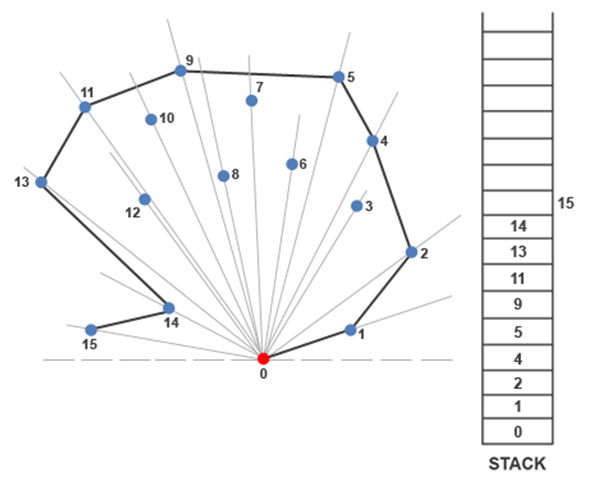
\includegraphics[width=0.6\linewidth]{latex/image/graham.png}
    \caption{Princíp fungovania Graham Scan}
    \label{fig:enter-label}
\end{figure}

\subsubsection*{Jarvis Scan}
Tento algoritmus je v odbornej literatúre označovaný aj ako Jarvis March, či Gift Wrapping Algorithm. Vo všeobecnosti platí, že je populárnou, jednoduchou a ľahko implementovateľnou metódou, ktorá má ale kvadratickú časovú záležitosť \(O(n^2)\), čo robí tento algoritmus neefektívny v komplexnej sade dát. Funguje systematickým obaľovaním sady bodov do najmenšieho možného konvexného mnohouholníka. Proces začína výberom počiatočného bodu (pivot \(q\)) ako súčasť konvexného obalu, $$ y_i=\min\limits_{\forall p_i \in S} .$$ \par Následne postupne pridáva nové body otáčaním okolo existujúcich bodov, pričom vyhledáva maximálny úhol \(\omega_{max}\) mezdi poslednou \((p_{j-1}, p_j)\) a nasledujúcou hranou \((p_j, p_{j+1})\) konvexní obálky. Na nájdenie bodu  \((p_{j+1})\) nasledujúcej hrany je potrebné prejsť všetky body, ktoré ešte nie sú súčasťou obálky (Bayer, 2024; Berg, 2008).
\begin{figure}[h]
    \centering
    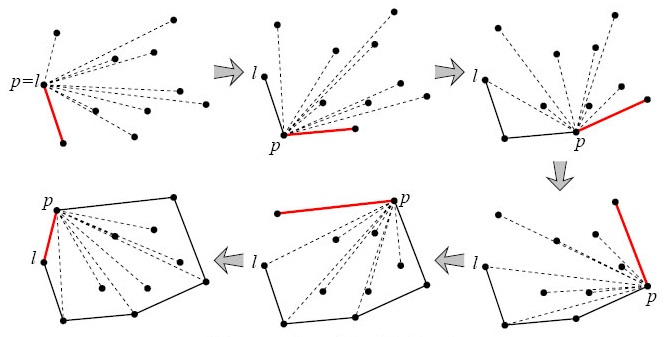
\includegraphics[width=0.6\linewidth]{latex/image/jarvis.jpg}
    \caption{Princíp Jarvis Scan}
    \label{fig:enter-label}
\end{figure}

\subsubsection*{Singulárne prípady}
Extrémne body množiny sú vrcholy konvexného obalu, kde je vnútorný uhol menší ako \( \pi \). Bod je extrémny vtedy, pokiaľ je možné vytvoriť medzi ním a všetkými ostatnými bodmi pomyselnú úsešku, ktorá nepretína konvexný obal (obsahujúci tento skúmaný bod). Počet extrémnych (vrcholových) bodov musí spĺňať nejaké parametre. Keďže potrebujeme vytvoriť polygón, a nie len priamku, tak na vznik polygónu (roviny) sú potrebné minimálne tri body(Rourke, 1997).
Okrem toho je potrebné definovať konvexný mnohouholník P, ktorého všetky vnútorné uhly sú konvexné a všetky jeho uhlopriešky ležia v jeho vnútri (Bayer, 2024).
\subsection*{Hlavný smer budov}
Hlavným problémom pri kartografickej generalizácii budov je zachovanie orientácie budovy. Pred a po generalizácii musí mať budova zachovanú orientáciu vzhľadom na ostatné prvky mapy, ako sú napríklad uličné čiary. Je nevyhnutné identifikovať tzv. hlavné smery budovy, ktoré sú navzájom kolmé a popisujú jej orientáciu. Uchovanie týchto informácií je kľúčové pre zachovanie čitateľnosti a interpretácie mapy, ako aj pre ďalšie aplikácie, ako je  analýza priestorových vzťahov. Detekcia a správne určenie hlavných smerov budovy prispieva k presnejšiemu a kvalitnejšiemu výsledku procesu generalizácie. Za týmto účelom bolo vytvorené viacero algoritmov, ktoré si následne podrobnejšie rozoberieme (Bayer, 2024).


\subsubsection*{Minimum Area Enclosing Rectangle}
Často označovaný aj ako Smallest area enclosing rectangle, spočíva v postupnom otáčaní obdĺžnika, ktorý sa zmenšuje (aproximuje) každým krokom, pokiaľ sa jeho plocha nezmenší natoľko, že sa stane najmenším obálkovým obdĺžnikom. Zároveň však platí, že jeho jedna hrana musí byť kolineárna s úsekom konvexného obalu. Pri tomto algoritme sa ale stretávame s numerickou nepresnosťou v dôsledku kumulácie chýb. Tieto chyby sú zapríčinené obdĺžnikovým tvarom budov (polygónov), v dôsledku čoho sú okraje obdĺžnika totožné s viacerými segmentmi konvexného obalu.\par
Algoritmus hľadá minimálny uhol $\varphi$, o ktorý bude obdĺžnik otočený. Tento uhol je zvieraný hranami najmenšieho obálkového obdĺžnika a hranami konvexného obalu v bode ich kontaktu $V_j$, ktorý je taktiež začiatkom kolineárneho segmentu. Pokiaľ nie je súčet týchto minimálnych uhlov menší ako $\frac{\pi}{2}$, tak porovnavame plochu obdĺžníkov s hodnotou minimálnej plocha inicializovanej do $\infty$, až kým na nenájde obdĺžnik s minimálnou plochou. Platí, že vrcholy ($M_j$) a hrany najmenšieho obálkového obdĺžnika sú orientované v smere hodinových ručičiek (Bayer, 2008).

\begin{figure} [h]
    \centering
    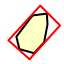
\includegraphics[width=0.62\linewidth]{latex/image/maer.png}
    \caption{Princíp Minimum Area Enclosing Rectangle}
    \label{fig:enter-label}
\end{figure}
\subsubsection*{PCA}
Analýza hlavných komponentov $(PCA)$ je metóda využívajúca strojové učenie na zjednodušenie veľkej dátovej sady na menšiu, pričom stále obsahuje väčšinu informácií o premenných z pôvodnej sady. Zníženie počtu premenných síce vedie ku menšej presnosti, čo sa ale vynahradí zjednodušením celej sady. Takéto dátové sady bez nepotrebných premenných sú ľahšie na prehľadávanie, čo zjednodušuje analýzu a urýchľuje proces algoritmov. Hlavné komponenty sú teda nové premenné, ktoré vznikli lineárnymi kombináciami pôvodných premenných. Informácie z pôvodných premenných sú najviac koncentrované v prvých komponentoch (Jaadi, 2024). Jeho nevýhodou je, že má nízku efektivitu pri pravidelných objektoch (štvorec, kružnica) (Bayer, 2024). 
\begin{figure}[h]
    \centering
    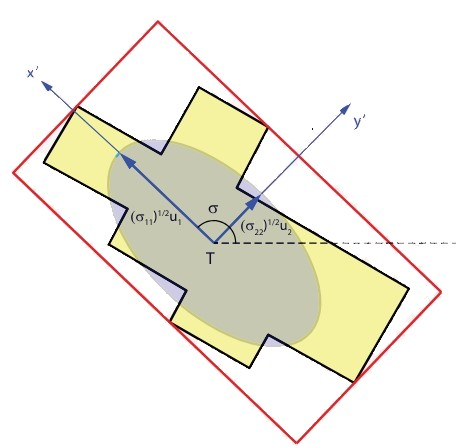
\includegraphics[width=0.56\linewidth]{latex/image/pca.jpg}
    \caption{Hlavný sme s využitím PCA}
    \label{fig:enter-label}
\end{figure}\par
Pre nájdenie hlavných smerov sa využívá singulárny rozklad $(SVD)$ na faktorizáciu kovariačnej matice do troch matíc. Kovariačná matica je simetrická ($p\times p$), kde p predstavuje počet dimenzií a jej úlohou je zistiť vzťahu medzi prvkami dátovej sady, pričom platí, že  $ C(A, B) = \frac{1}{n-1}\sum_{i=1}^{n}(A_{i}-\mu_{A}) -(b_{i}-\mu_{B}), $
$$$$$$
  C =
  \left[ {\begin{array}{cc} 
    C(A, A) & C(A, B) \\
    C(B, A) & C(B, B) \\
  \end{array} } \right].
$$ \\\par
Singulárnym rozkladom tak dostaneme $C = U\sum V^T$, čo sa dá rozpísať následovne,
$$$$$$
\left[ {\begin{array}{cc} 
    C_{11} & C_{12} \\
    C_{21} & C_{22} \\
\end{array} } \right]
=
\left[ {\begin{array}{cc} 
    u_{11} & u_{12} \\
    u_{11} & u_{12}\\
  \end{array} } \right] 
  \left[ {\begin{array}{cc} 
    \sigma_1 & 0 \\
    0 & \sigma_2 \\
  \end{array} } \right]
  \left[ {\begin{array}{cc} 
    v_{11} & v_{12} \\
    v_{11} & v_{12}\\
  \end{array} } \right]. 
$$\\ \par
Matica $U$ predstavuje vlastné vektory $C\cdot C^T$, matica $V^T$ taktiež vlastné vektory $C^T\cdot C$ a matica $\sum$ veľkosť vlastných vektorov (singulárne hodnoty),
$$ $$$$U = V \equiv 
\left[ {\begin{array}{cc} 
    cos\sigma & - sin\sigma \\
    sin\sigma & cos\sigma\\
  \end{array} } \right],
$$$$$$
$$
  \sum =
  \left[ {\begin{array}{cc} 
    \sigma_1 & 0 \\
    0 & \sigma_2\\
  \end{array} } \right]
  =
  \left[ {\begin{array}{cc} 
    \sqrt{\lambda_1} & 0 \\
    0 & \sqrt{\lambda_2}\\
  \end{array} } \right].
\par
Množina P sa následne otočí o uhol $\pm\omega$ pričom platí, $$P_{0}= P\cdot V,$$  $$ P = V^{-1}\cdot P_. $$

\newpage

\subsubsection*{Wall Average}
Táto metóda je pomerne robustná vzhľadom na rôzne tvary budov a ich stien. Avšak je citlivá na uhly, ktoré sú veľmi odlišné od hlavných orientácií.  Podĺa Bayera (2024) sa najprv určia smernice všetkých hrán a vypočítajú sa v každom vrchole vnútorné uhly $\omega_{i}=|\sigma_{i,i-1}-\sigma_{i,i+1}|$ medzi smernicou a hranou. Následne sa aplikuje operácia mod($\frac{\pi}{2}$), vďaka čomu je každá strana budovy zarovnaná za účelom zjednodušej geometrickej analýzy a porovnávania stien.\par  Dostaneme tak vzťah $k_{i}=\frac{2*\omega_{i}}{\pi}$, ktorý sa ďalej použije na zistenie orientovaného zvyšku po delení podľa vzorca $r_{i} = (k_{i} - \lfloor k_{i} \rfloor)*\frac{\pi}{2} $. Nakoniec sa na určenie hlavného smeru budovy vypočíta vážený priemer, do ktorého stupuje orientovaný zvyšok a váhy ($s_{i}$) v podobne dĺžky jednotlivých strán budovy, $$ \sigma = \sigma_{1, 2} + \sum_{i=1}^{n}\frac{r_{i}s_{i}}{s_{i}}. $$   
\begin{figure} [h]
    \centering
    
\includegraphics[width=1\linewidth]{latex/image/wa.png}
    \caption{Znazornenie Wall Average}
    \label{fig:enter-label}
\end{figure}
\newpage
\subsubsection*{Weight Bisector}
Bayer (2024) uvádza, že Weighted Bisector algoritmus je používaný pre hľadaníe hlavného smeru objektu v rovine pomocou dvoch najdlhších uhlopriečok, ktoré nepretetínajú hranice polygónu. Pri jeho výpočte do rovnice váženého priemeru vstupujú smernice $(\sigma_{1}, \sigma_{2})$    a dĺžky týchto uhlopriečok $(S_1, S_2)$, ktoré predstavujú váhy, 
$$\sigma = \frac{S_1*\sigma_1 + S_2*\sigma_2}{(S_1+S_2)}.$$
\begin{figure}[h]
    \centering
    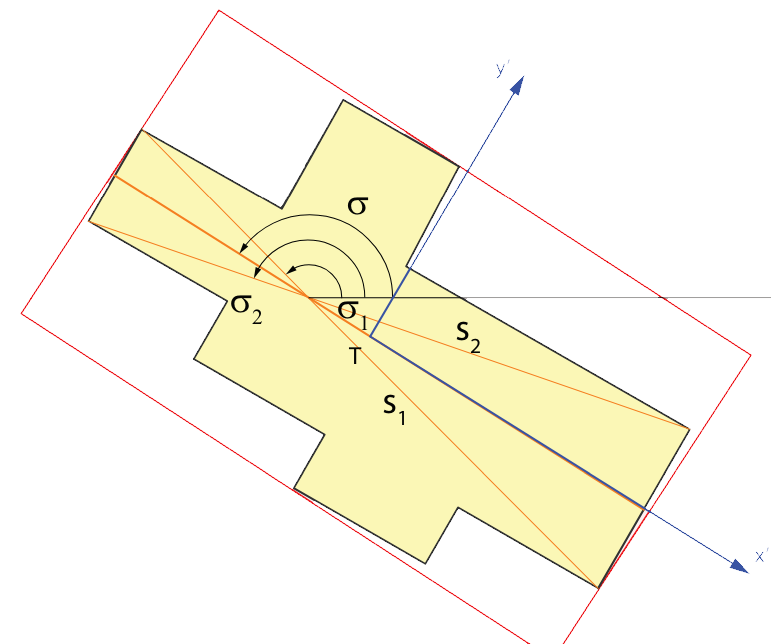
\includegraphics[width=0.7\linewidth]{latex/image/wb.png}
    \caption{Princím Weight Bisector}
    \label{fig:enter-label}
\end{figure}
\subsubsection*{Longest Edge}
Prvý hlavný smer budovy je určený najdlhšou stranou budovy, druhý hlavný smer je na ňu kolmý. Táto metóda však nedosahuje príliš dobrých výsledkov. Je to zapríčinené tým, že najdlhšia strana nemusí vždy reprezentovať hlavný smer. Na druhej strane ale poskytuje určité indikácie o jej tvare a orientácii (Bayer, 2024). 
\begin{figure}[t]
    \centering
    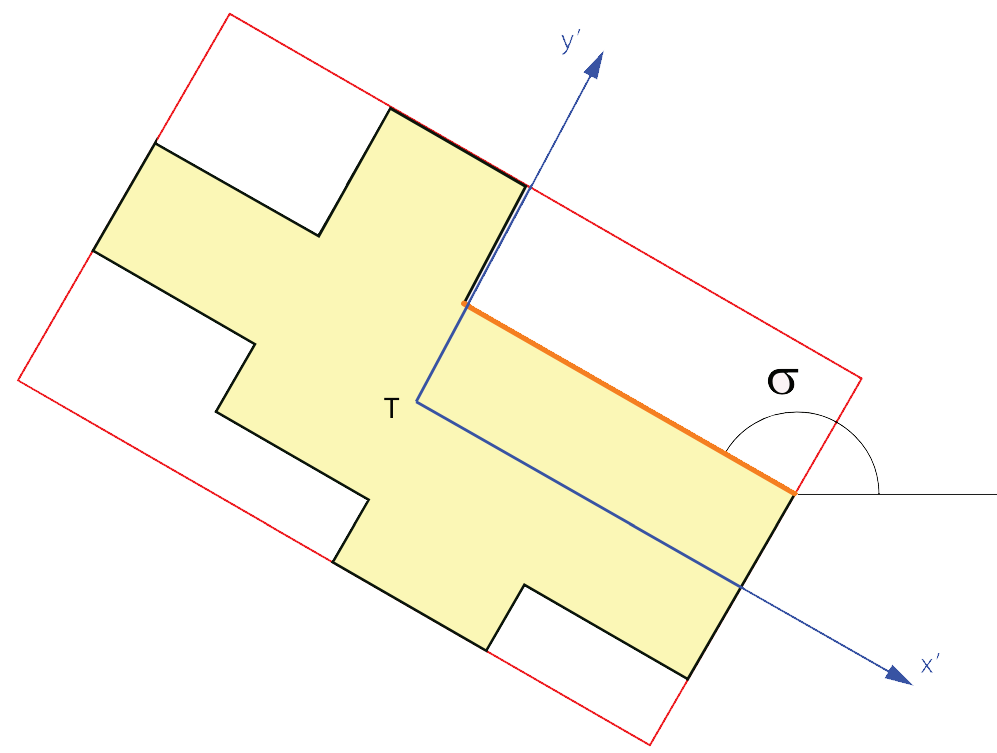
\includegraphics[width=0.7\linewidth]{latex/image/le.png}
    \caption{Longest Edge algorimus}
    \label{fig:enter-label}
\end{figure}
\newpage
\section*{Implementovanie}
Po priblížení problematiky a vysvetlení metód na jej riešenie je ďalším krokom v tomto zadaní tvorba užívateľského prostredia, v ktorom bude možné demonštrovať  rôzne prístupy ku generalizovaniu tvaru budov v troch rôznych lokalitách. Tieto lokality sa od seba odlišujú hustotou, ale aj komplexnosťou tvaru budov. Pre dataset historickej časti mesta bola zvolená Horná ulica v Banskej Bystrici (BB), pre intravilán (sídlisko) bolo v rámci BB vybrané Uhlisko a ako zdroj budov v izolovanej zástavbe bola oblasť lazov nad Hriňovou, ktoré predstavujú roztrúsenú sídelnú zástavbu.
\subsection*{Vstupné dáta}
Naše dáta bolo možné získať v troch rôznych formátoch (ESRI GDB, GML a GeoPackage) zo stranky geoportálu. Dátová sada INSPIRE - Budovy je súčasťou celoslovenskej geografickej databázy ZBGIS. Vytvorenie ZBGIS prebieha v troch fázach: fotogrametrické vyhodnotenie leteckých snímok, doplnenie, ale aj revidovanie v teréne a kontrola kvality podľa ISO noriem. Kvalita údajov je definovaná presnosťou geometrie, správnosťou atribútov, kompletnosťou a topológiou. Geometrické dáta môžu byť získavané geodetickými alebo fotogrametrickými metódami, pričom sa preferuje presnejšia metóda.
\par Druhým alternatývnym zdrojom dát by mohol byť Google Earth Engine, kde bolo možné získať Microsoft Building Footprint Data. Obrysy budov boli vytvorené použitím hlbokým neurónovým sieťam a AI zo záznamov Bing, pričom bol využitý algoritmus na polygonizáciu. Nevyhoda týchto dát bola v tom, že pre územie historickej časti mesta zhlukovala budovi do jedného, veľmi nerealistickkého polygónu. Ďalej treba spomenúť, že v Google Earth Engine je potrebné dodatatočné programovanie. 

\begin{figure}[h]
    \centering
    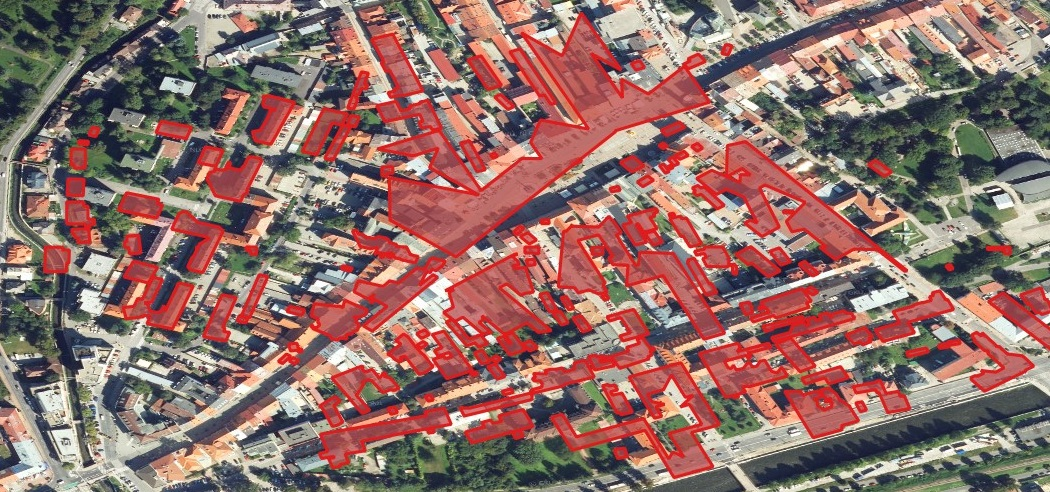
\includegraphics[width=0.7\linewidth]{latex/image/chyba.jpg}
    \caption{Chybné polygóny budov v historickej časti mesta}
    \label{fig:enter-label}
\end{figure}\par
Keďže stiahnuté dáta obsahovali všetky budovy v republike, tak ich bolo potrebné vyfiltrovať iba na územie nášho záujmu. Za týmto účelom boli vytvorené 3 polygónové vrstvy v oblasti Hriňovských lazov, Uhliska (BB) a Námestia SNP (BB). Následne sme pomocou funkcie intersect vybrali len tie budovy, ktoré boli prienikom naších dvoch vrstiev. Súradnice boli v súradnicovom systéme WGS84 a bolo ich potrebné transformovať na S-JTSK. To bolo docielené zvolením súradnicového systému pri exportovaní naších budov do GeoJSON.
\begin{figure}[h]
    \centering
    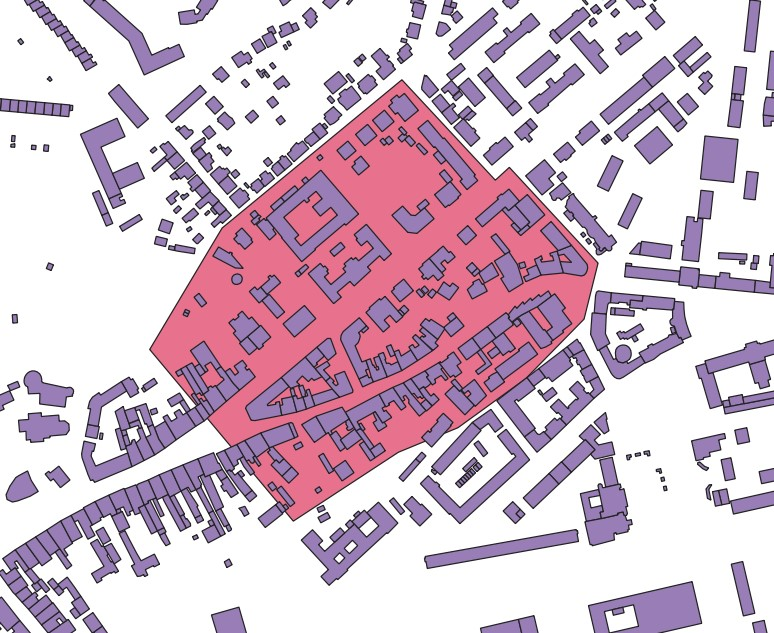
\includegraphics[width=0.7\linewidth]{latex/image/filter.jpg}
    \caption{Filtrovanie budov}
    \label{fig:enter-label}
\end{figure}
\newpage
\subsection*{Aplikácia}
Grafické užívateľské prostredie (GUI) aplikácie  pozostávalo z okna, lišty a panelu obsahujúceho ikony, ktoré bolo vytvorené za pomoci knižnice QT (v.4.6.1) a jeho funkcionalita bolo ďalej doplňovaná za pomoci programovacieho jazyka Python 3.11. Vďaka tomu bolo možné pre jednotlivé ikony pridať aj ich funkcie.

\begin{figure} [h]
    \centering
    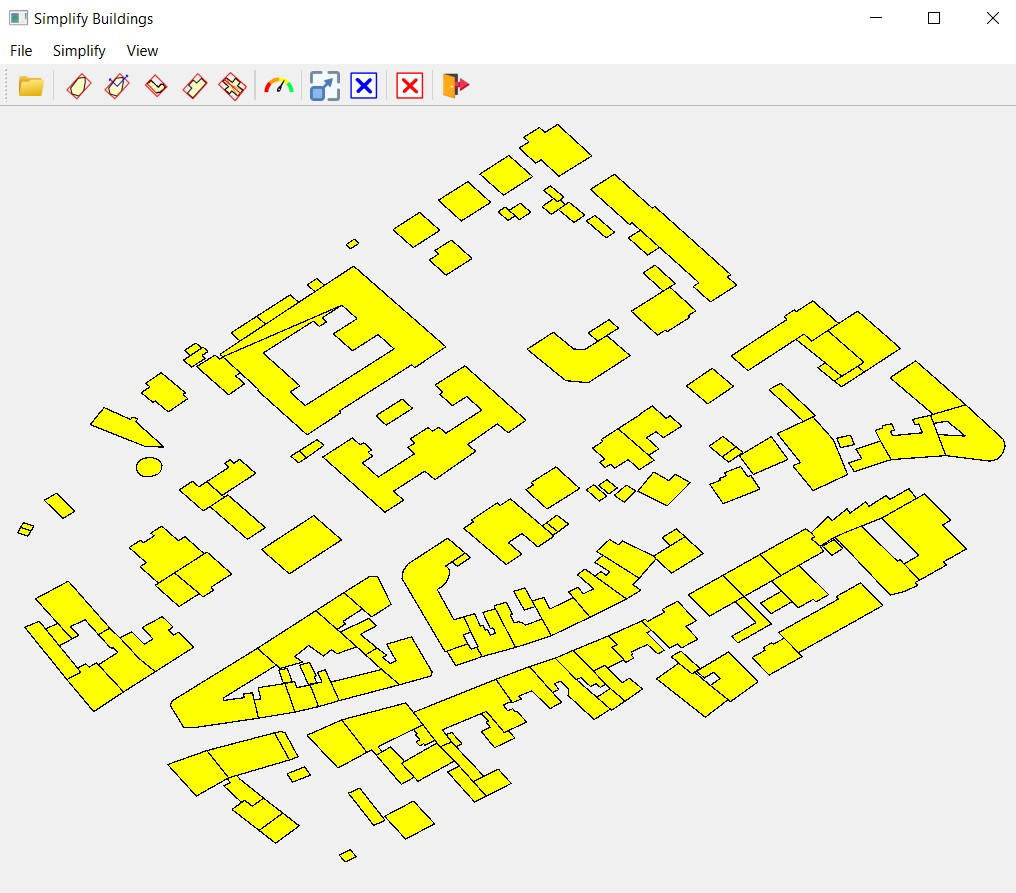
\includegraphics[width=0.5\linewidth]{latex/image/apka.jpg}
    \caption{GUI aplikácie}
    \label{fig:enter-label}
\end{figure}
Celkovo bolo použitých 11 ikon (obr. 6), ktorých úlohou je urýchliť prácu používateľa, 
vďaka čomu nie je potrebné prechádzať lištu a hľadať jednotlivé procesy, ktoré by sme pri 
väčšej komplexnosti aplikácie mohli prehliadnuť. \\

\begin{figure}[h]
    \centering
    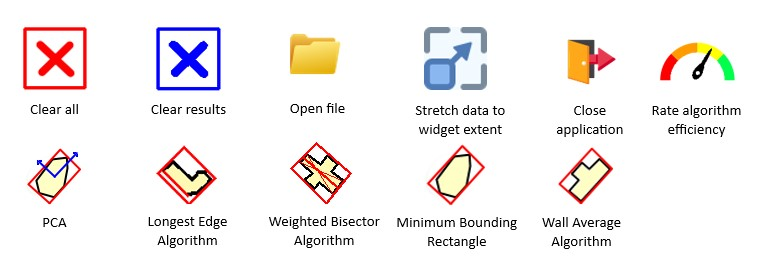
\includegraphics[width=0.7\linewidth]{latex/image/icons.jpg}
    \caption{Význam jednotlivých ikon}
    \label{fig:enter-label}
\end{figure}
Aplikácia dáva používateľovi na výber z piatich analytických metód, ktoré sa spustia 
hneď po kliknutí na príslušnú ikonu. Keď sa používateľ rozhodne pre použitie iného algoritmu, tak sa výsledky automaticky preklesia. Po spustení algoritmu vybehne  pop-up okna s textom, či bolo možné uskutočníť našu metódu na všetkých budovách. Okrem toho pop-up okno slúži aj na zobrazenie efektivity detekcie hlavných smerov a po zatvorení okna sa vygeneruje tabuľka, ktorú je možné s týmito hodnotami vyexportovať.  


\begin{figure}[h]
    \centering
    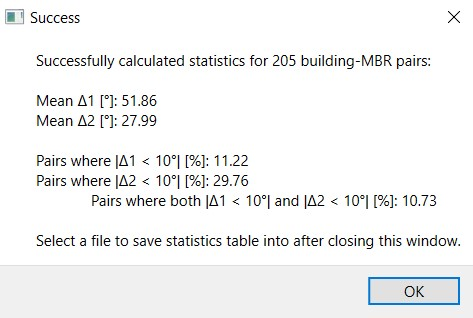
\includegraphics[width=0.5\linewidth]{latex/image/success.jpg}
    \caption{Celkové hodnotenie algoritmu na sade dát}
    \label{fig:enter-label}
\end{figure}

\subsection*{Výstupné dáta}
Polygóny vykreslené v aplikácii nie je možné exportovať. Miesto toho je možné vyexportovať tabuľku obsahujúcú hodnoty uhlovej odchýlky ($\Delta\sigma_{1}$) a hodnotu uhlovej odchýlky vo štvorcoch ($\Delta\sigma_{2}$) v textovom formáte. 
\begin{figure}[h]
    \centering
    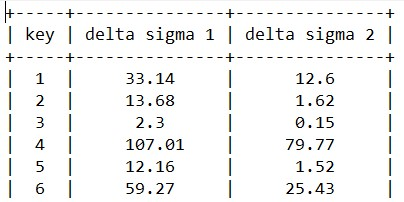
\includegraphics[width=0.5\linewidth]{latex/image/tabulka.jpg}
    \caption{Exportovaná tabuľka}
    \label{fig:enter-label}
\end{figure}
\newpage
\section*{Dokumentácia}
\subsection*{Trieda Ui\textunderscore MainWindow}
Trieda UiMainWindow je zodpovedná za celé GUI, ktoré pozostáva z okna, widget
a lišty, na ktorej sa nachádzajú ikonky pre zjednodušené ovládanie. Nachádzajú sa tu okrem toho prepojenia jednotlivých ikon s ich funkcionalitami v iných triedach. Funkcie setupUi (), retranslateUI () boli vytvorené automaticky QT.
\subsubsection*{openClick()}
\noindent-načíta údaje o polygóne zvolené zvolením súboru cez dialógové okno súboru
\subsubsection*{generalizationProcess(algo: Callable, algo\textunderscore name: str)}
\noindent-overí, či sú údaje použiteľné, pripraví ich, zavolá daný algoritmus MBR, aktualizuje uložené údaje, používané 5 metódami v triede Algorithms.

\subsubsection*{ratingClick()}
\noindent-vypočíta efektivitu detekcie hlavného smeru počítača, zobrazí jeho štatistiky a uloží tabuľku štatistík do súboru vybraného pomocou dialógového okna súboru
\subsubsection*{rescaleClick()}
\noindent-zmení aktuálne údaje o polygóne na veľkosť okna
\subsubsection*{clearAllClick()}
\noindent-vyčistí všetky údaje z Canvas a pamäte programu
\subsubsection*{clearResClick()}
\noindent-vymaže iba výsledky
\subsubsection*{exitClick()}
\noindent-ukončí program
\subsection*{Trieda IO}
Funkcie v tejto triede spracovávajú operácie zodpovedné za načítanie a ukladanie dát. Dialógové okno dovolí načítať v GeoJSON fomátovaní súbori len s koncovkou *.GeoJSON, *.JSON a *.TXT. Je potrebné, aby tieto dáta boli v S-JTSK (EPSG:5514). 
\subsubsection*{readPnts(pnt\textunderscore list: list)}
\noindent-vytvára zoznam n-tíc súradníc
\subsubsection*{loadBlds(file: str, width: int, height: int)}
\noindent-načíta dáta zo súboru a preškáluje dáta podľa veľkosti widget
\subsubsection*{saveTable(file: str, table: PrettyTable)}
\noindent-uloží tabuľku štatistík účinnosti hlavného smeru a vráti hodnotu typu bool o výsledku ukladania
\subsection*{Trieda Draw}
Metódy v tejto triede sú zodpovedné za interakciu používateľa s grafickým užívateľským rozhraním a manipuláciu s vykresľovaním a analýzou objektov. Taktiež obsahuje funkcie typu getter a setter.
\subsubsection*{\textunderscore \textunderscore init\textunderscore \textunderscore(*args, **kwargs)}
\noindent-konštruktor s predvolenými parametrami potrebnými pre Qt, nastavuje rámec pre kreslenie na widgete
\subsubsection*{mousePressEvent(e: QMouseEvent)}
\noindent-eaguje na kliknutie myšou na widget, čo má za následok vykreslenie testovaného bodu alebo bodu do polygónu
\subsubsection*{paintEvent(e: QPaintEvent)}
\noindent-obnovuje widget
\subsubsection*{messageBox(title: str, text : str)}
\noindent-vytvára dialógové okno s daným textom
\subsubsection*{clearData()}
\noindent-nastaví dáta rámca pre kreslenie na predvolené hodnoty
\subsubsection*{clearMBRs()}
\noindent-odstráni minimálne ohraničujúce obdĺžniky (MBR)
\subsection*{Trieda Algorithms}
Táto trieda implementuje geometrické algoritmy na prácu s polygónmi, so zameraním sa najmä na hľadanie najmenších ohraničujúcich obdĺžnikov (MBR) pre dané polygóny. Na to je potrebné najprv tieto algoritmy definovať, priradiť ku ním ďalšie pomocné metódy (napr. výpočet ulov/plôch), či odstránenie duplicitných bodov. Okrem toho sa tu nachádzajú aj dve výnimky. Prvá ošetruje prípady, kedy budova má menej ako 3 body a druhá zavolálo Error, keď MAER algoritmus spadne. Taktiež sa tu rieši hodnotenie jednotlivých algoritmov a prevod súradníc medzi súradnicovými systémami.
\subsubsection*{generalize(algo : Callable, blds : dict)}
\noindent-volá zadaný algoritmus na vytvorenie MBR pre každú predspracovanú budovu, pokiaľ má jej polygón aspoň tri body. 
\subsubsection*{MAER(bld : QPolygonF)}
\noindent-používa Graham scan algoritmus na vytvorenie konvexnej obálky
\subsubsection*{PCA(bld : QPolygonF)}
\noindent-výpočet MBR pomocou metódy Principal Component Analysis
\subsubsection*{LE(bld : QPolygonF)}
\noindent-výpočet MBR pomocou metódy Longest Edge algorithm
\subsubsection*{WA(bld : QPolygonF)}
\noindent-výpočet MBR pomocou metódy Wall Average algorithm
\subsubsection*{WB(bld : QPolygonF)}
\noindent-výpočet MBR pomocou metódy Weighted bisector algorithm
\subsubsection*{LE\textunderscore Sigma(bld : QPolygonF)}
\noindent-nájde najdlhšiu hranu budovy a jej sigma, používané algoritmom Longest Edge
\subsubsection*{MBR\textunderscore FromSigma(bld : QPolygonF, sigma : float)}
\noindent-vytvorí MBR z danej budovy a jej sigma, používané vo všetkých algoritmoch MBR
\subsubsection*{innerDiags(bld : QPolygonF, diags : dict)}
\noindent-triedi diagonály danej budovy do kolekcií diagonál vnútri / mimo danej budovy, používané algoritmom Weighted Bisector
\subsubsection*{windingNum(bld: QPolygonF, q: QPointF)}
\noindent-spúšťa algoritmus Winding Number pre danú budovu a bod, vráti pozitívny výsledok len v prípade, že bod nie je mimo, na hrane budovy alebo nie je rovnaký ako vrchol budovy
\subsubsection*{rateAll(blds : dict, mbrs : dict, common\textunderscorek : set)}
\noindent-vypočíta efektivitu detekcie hlavného smeru MBR pre každú kombináciu budovy-MBR.
\subsubsection*{rateSingle(bld : QPolygonF, mbr : QPolygonF)}
\noindent-vypočíta efektivitu pre jednotlivú kombináciu budovy-MBR
\subsubsection*{R(sig : float)}
\noindent-vypočíta konštantu R z daného sigma MBR, používaného na porovnanie s budovou v metóde rateSingle()
\subsubsection*{fineCount(values : list)}
\noindent-vráti počet hodnôt v zozname nižších ako 10, používané v algoritme na hodnotenie efektivity
\subsubsection*{grahamScan(bld : QPolygonF)}
\noindent-vypočíta konvexný obal pomocou algoritmu Graham Scan a vráti striktný konvexný obal
\subsubsection*{get\textunderscore 2line\textunderscore angle(p\textunderscore from : QPointF, p\textunderscore to : QPointF, p\textunderscore from1 : QPointF, p\textunderscore to1: QPointF) }
\noindent-vypočíta uhol dvoch úsečiek v radiánoch
\subsubsection*{starShapedPolygon(bld: QPolygonF)}
\noindent-vytvorí hviezdicový polygon z vstupnej budovy a odstráni duplicitný bod, ak majú dva susedné body rovnaký uhol
\subsubsection*{rotate(mmb : QPolygonF | tuple, sig : float)}
\noindent-otočí danú Min-Max Box o daný uhol
\subsubsection*{setInputPol(pol : QPolygonF | tuple)}
\noindent-vytvorí CCW orientovaný QPolygonF z daného Min-Max Boxu
\subsubsection*{getArea(bld : QPolygonF | tuple)}
\noindent-vypočíta plochu vstupných budov
\subsubsection*{resizeRect(mmb: QPolygonF, build: QPolygonF)}
\noindent-zmenší daný Min-Max Box, aby sa zhodoval s plochou vstupnej budovy
\subsubsection*{setCCW\textunderscore Orientation(blds : dict)}
\noindent-testuje rotáciu každého polygónu, nastaví ju na proti smeru hodinových ručičiek (CCW), pokiaľ tak nie je
\subsubsection*{removeDupl(blds : dict)}
\noindent-vráti danú budovu s jedinečnými bodmi
\subsubsection*{strictC\textunderscore Hull(ch : QPolygonF)}
\noindent-transformuje daný konvexný obal na prísny konvexný obal
\subsubsection*{halfPlaneTest(p\textunderscore from : QPointF, p\textunderscore to: QPointF, p\textunderscore test: QPointF)}
\noindent-vráti determinant testu polovice r

\subsubsection*{minMaxBox(polygon: QPolygonF | list)}
\noindent-vytvorí Min-Max Box vstupnej budovy
\subsubsection*{coordDiffDist(p1 : QPointF, p2 : QPointF)}
\noindent-vypočíta vzdialenosť súradníc v každej dimenzii a ich euklidovskú vzdialenosť
\subsubsection*{sjtsk2Pixel(point : list, width : int, height : int, x\textunderscore min : float, x\textunderscore max : float, y\textunderscore min : float, y\textunderscore max : float)}
\noindent-konvertuje súradnice S-JTSK CRS (EPSG: 5514) na pixelové súradnice
\subsubsection*{rescaleAll(blds : dict, mbrs : dict, w : int, h : int)}
\noindent-na základe nových rozmerov preškáluje budovy a MBR, aby sa zmestili do widgetu s  posunom 5 pixelov
\newpage
\section*{Výsledky}
Na všetky naše datasety boli aplikované algoritmy za účelom detekovania hlavných smerov budov. V tejto časti si popíšeme výsledky jednotlivých algoritmov, koré budú ako kvalitatívneho, tak aj kvantitatívneho charakteru. Pri testovaní algoritmov sa hľadelo na ich schopnosť presne identifikovať hlavný smer v rôznych podmienkach. Vďaka tomu je možné určiť výhody, ale aj slabiny jednotlivých algoritmov, čo je dôležité do budúcna pri výber vhodného algoritmu pre nejaký dataset.
\subsection*{Dataset Horná}
Horná ulica je súčasťou historickej časti mesta, pre ktorú je typická súvislá, na seba často nadvädzujúca zástavba. Budovy tu majú v menšom množstve jednoduchý, ale prevažne komplexný, nekonvexný a veľmi nepraidelný pôdorys. Taktiež sa tu nachádza kruhový pôdorys bašty (historická strážna veža), ale aj pôdoris s vnútorným prsteňom pri väznici. Po väznici má najkomplikovanejší pôdoris budova súdu.

\par
Algoritmus MAER dokázal najlepšie generalizovať najzložitejšie budovy (súd a väznica) a takisto aj jednoduché a pravidelné budovy. V našom prípade ale nedokázal vytvoriť MBR akolo všetkých budov. PCA má dobré výsledky pri rohových budovách, ktoré sa často prejavujú zaobleným rohom. Naopak, čím jednoduchší a pravidelnejší pôdorys budovy (štvorec), tým horší výsledok. Longest Edge má veľmi podobné výsledky ako PCA, avšak pri jednoduchých tvaroch budov má veľmi dobré výsledky. Algoritmus Wall Average dokázal dobre generalizovať väznicu, ale problém mu trochu robili otočené budovy. Weight Bisector sa javý ako najhorší algoritmus pre túto sadu. Výsledky pri komplexnýxh budovách má podobné ako PCA, ale jednoduché budovy generalizuje ešte horšie.
\begin{figure}[h]
    \centering
    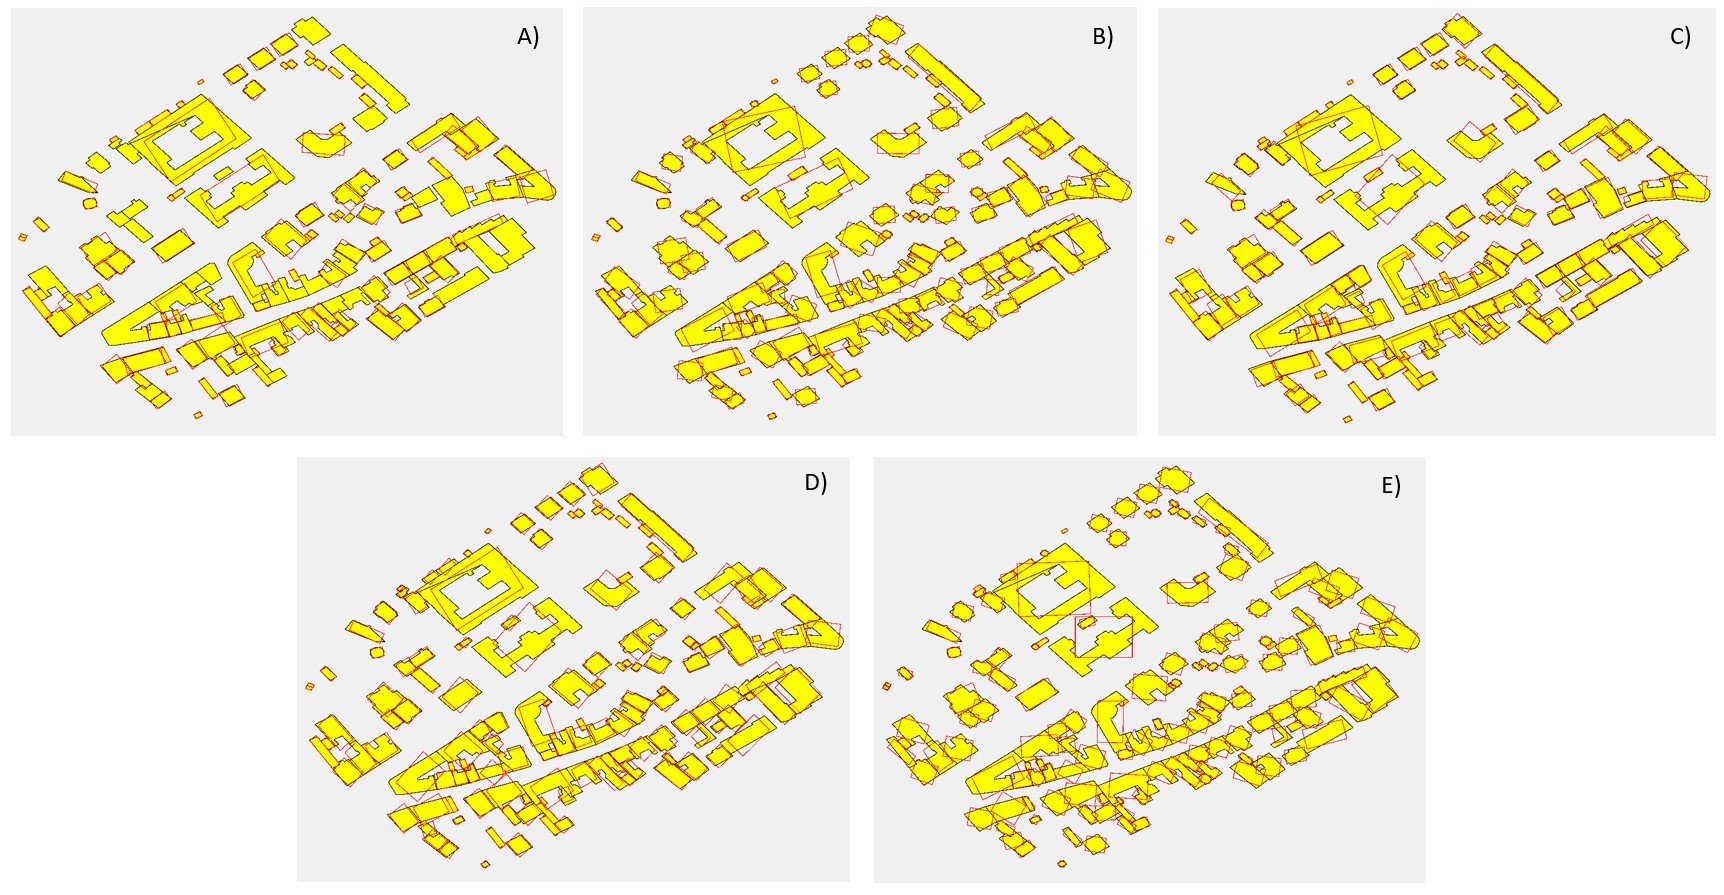
\includegraphics[width=1\linewidth]{latex/image/horna.jpg}
    \captionsetup{Figure 16: Porovnanie algoritmuv na dátovej sade Horná:\textit{ MAER (A), PCA (B), Longest Edge (C), Wall Average (D), Weight Bisector (E)} }
    \label{fig:enter-label}
\end{figure}
$$$$ 
\subsection*{Dataset Uhlisko}
Uhlisko je sídlisko, ktoré okrem panelových domov pozostáva aj z rodinných domov. Pôdorysy budov sú oveľa jednoduchšie ako v prípade Hornej ulice a celková hustota zástavby je tu nižšia. Podiel konvexných a nekonvexných tvarov pôdorysu sa javý byť veľmi podobný. Taktiež sa tu nájdu nadvezujúce pôdorysy väčšinou pravidelného tvaru a jedná sa hlavne o garáže, či iné prístavby ku rodinnym domom. .
\par
Väčšie množstvo budov mali podlhovastý tvar, ktorý dokázali algoritmy MAER, PCA a Longest Edge generalizovať veľmi dobre. Netreba však zabudnúť, že MAER opäť nebol schopný generalizovať všetky budovy a PCA mala opätovne problém pri pravidelných tvaroch, ale teraz v menšom množstve. Pre tento tvar budov sa javý byť najhorší Wall Average. Garáže predstavovali podlhovastý pôdorysrôdorys (tvar schodov), ktorý nedokázali dobre generalizovať Wall Average ani Longest Edge. V tejto sade ukázal potenciál Weight Bisector a jeho výsledky boli dramaticky lepšie ako pri sade Horná. Problémy mu ale robili kosodĺžniky.Ak odmyslíme generalizovanie garáží, tak Longest Edge sa javý byť ako najlepšia metóda pre generalizovanie tejto sady.
\begin{figure}[h]
    \centering
    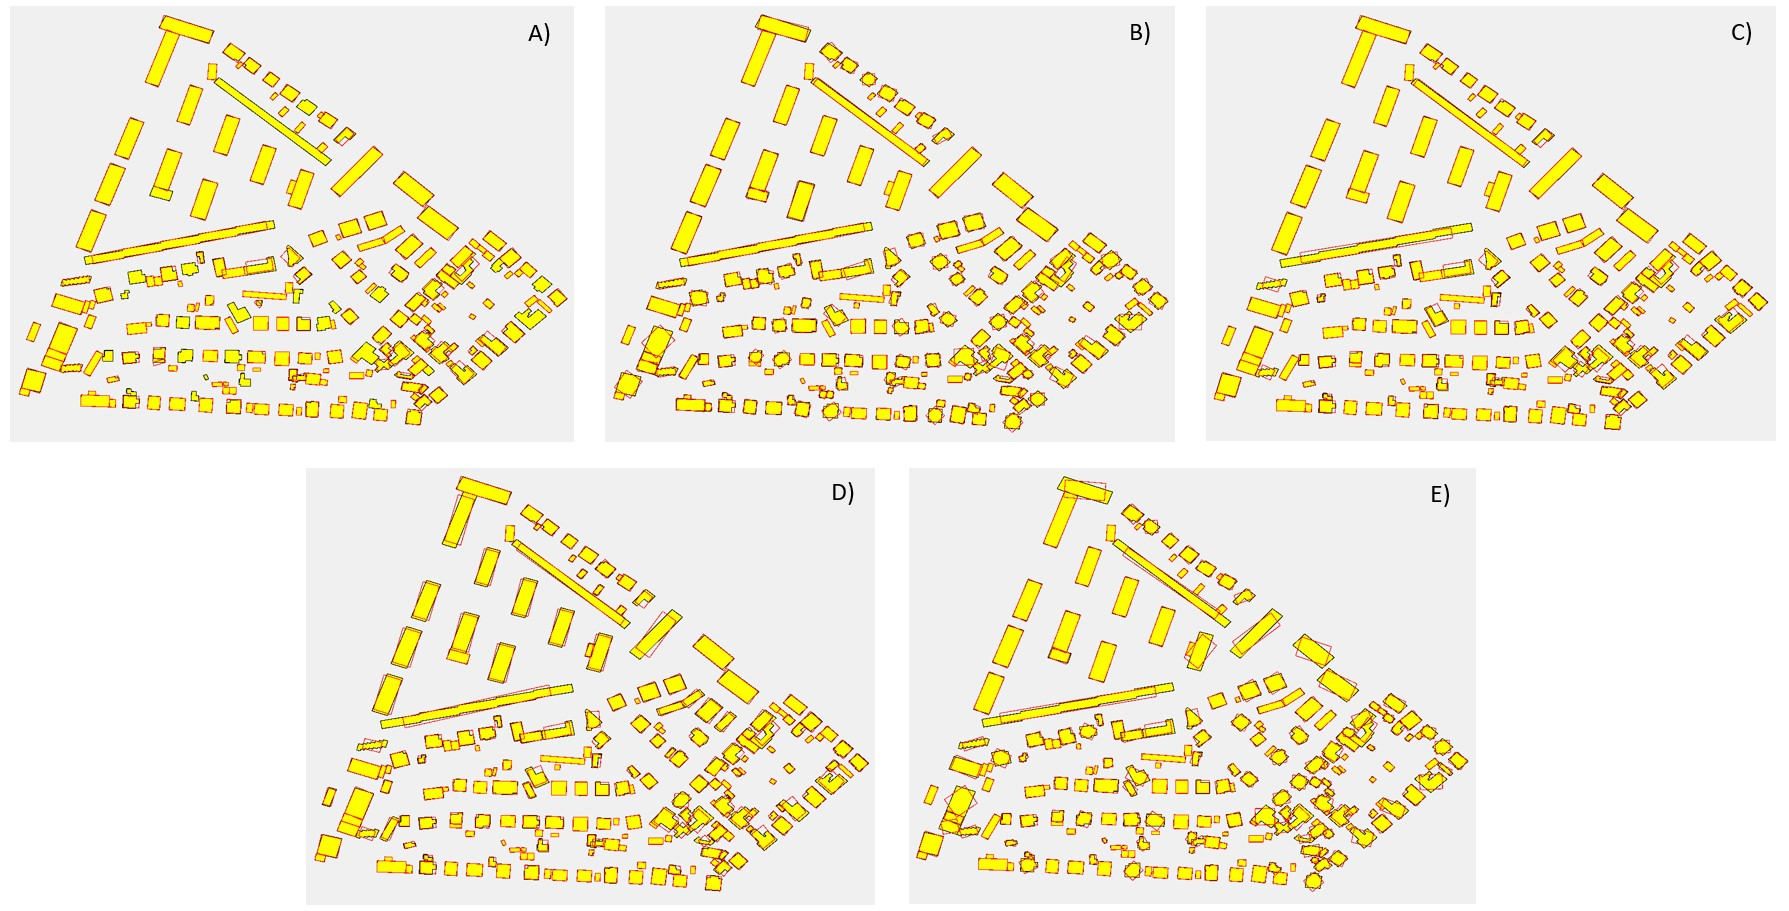
\includegraphics[width=1\linewidth]{latex/image/uhlisko.jpg}
    {Figure 17: Porovnanie algoritmuv na dátovej sade Uhlisko:\textit{ MAER (A), PCA (B), Longest Edge (C), Wall Average (D), Weight Bisector (E)} }
    \label{fig:enter-label}
\end{figure}
$$$$
\subsection*{Dataset Lazy}
Lazy predstavujú roztrúsené osídlenia v horskej oblasti. Z toho dôvodu je hustota zástavby oveľa nižšia a komplexnosť tvaru budov oveľa jednoduchšia ako v predchádzajúcich dvoch datasetoch. Taktiež sú tu na seba nadväzujúce polygoný predstavujúce prístavby ku domom, prípadne sa jedná o zlu segmentáciu dudovy. \par
Budovy tu majú prevažne jednoduchý tvar a zopár z ních sa podobá písmenu L. To robilo problém pre algoritmy Longest Edge a Weight Bisector. Podobne ako v predchádzajúcich datasetoch, tak aj tu má PCA problémy pôdorysmi v tvare štvorcov. Zvyšné algoritmy sa na prvý pohľad javia mať dobré výsledky.
\begin{figure}[h]
    \centering
    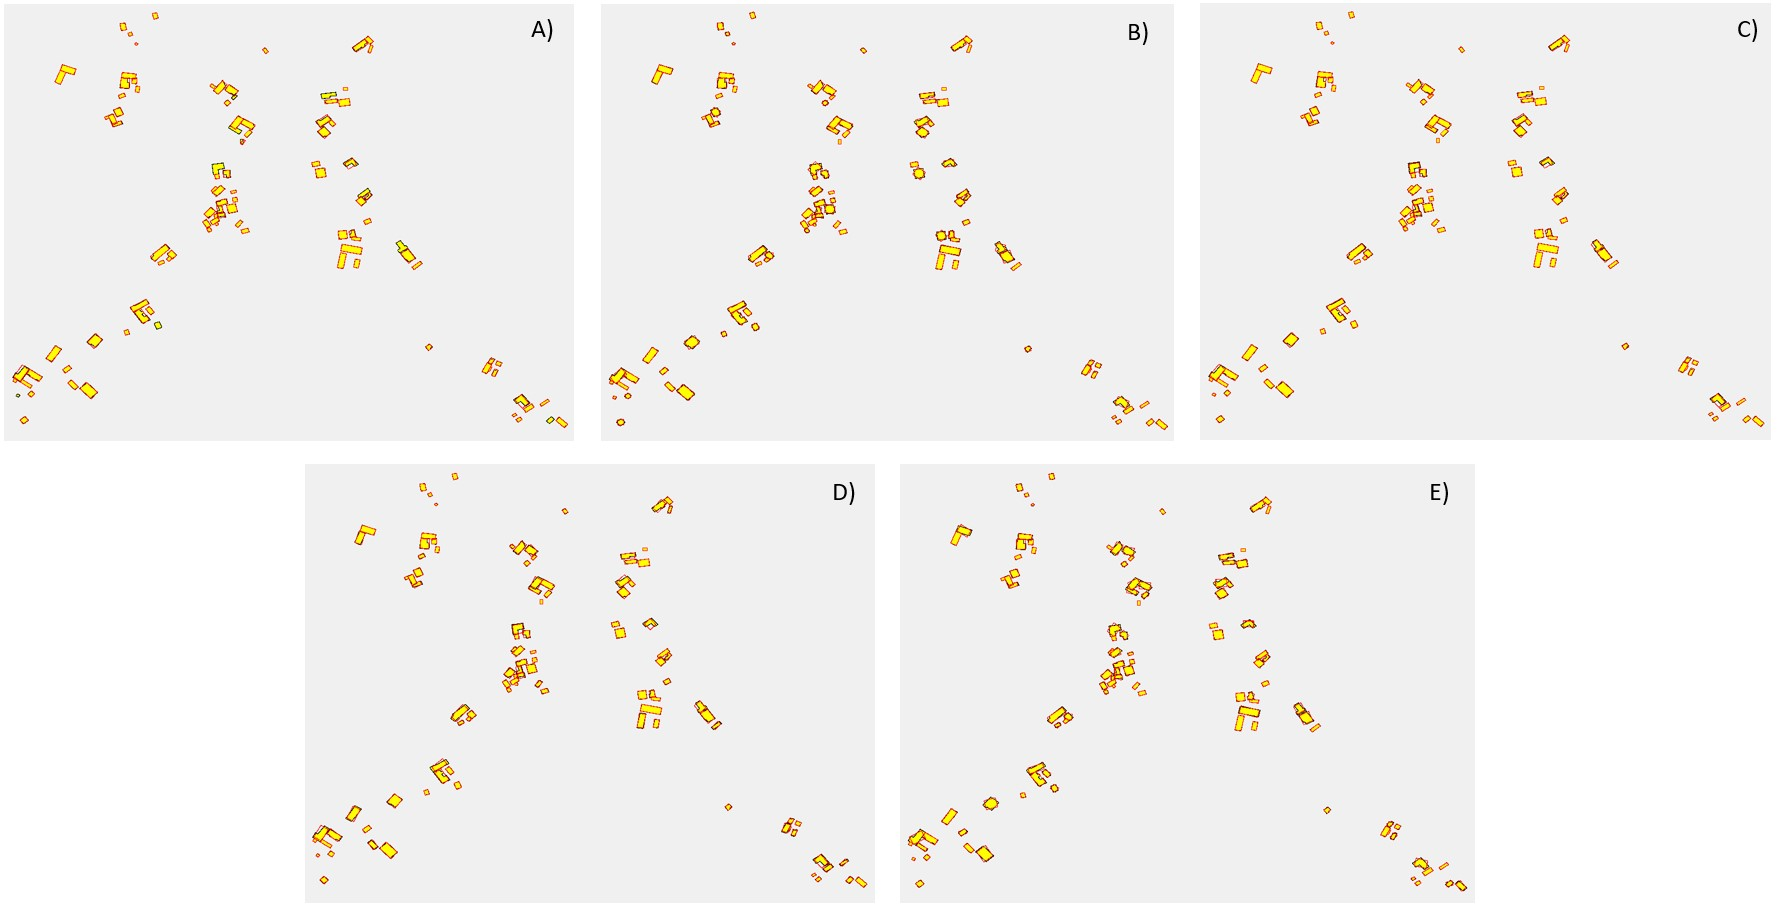
\includegraphics[width=1\linewidth]{latex/image/lazy.jpg}
    \captionsetup{Figure 18: Porovnanie algoritmuv na dátovej sade Lazy:\textit{MAER (A), PCA (B), Longest Edge (C), Wall Average (D), Weight Bisector (E)} }
     \label{fig:enter-label}
\end{figure}
$$$$
\subsection*{Zhrnutie výsledkov}
Kvalitatívny spôsob hodnotenia výsledkov nie je objektívny a je potrebné sa pozrieť na výsledky v číslach. Za týmto účelom boli vypočítané hodnoty uhlovej odchýlky ($\Delta\sigma_{1}$) a hodnotu uhlovej odchýlky vo štvorcoch ($\Delta\sigma_{2}$), pričom v praxi sa akceptovatujú objekty s hodnotou tohto uhla menšieho ako 10. Tento údaj bol následne vyjadrený aj v percentách (podiel párov splňujúcich túto podmienku).

$$ \Delta\sigma_{1} = \frac{\pi}{2n} \sum_{i=1}^{n}\left[ r_{i}-r \right], $$
$$ \Delta\sigma_{2} = \frac{\pi}{2n} \sqrt{\sum_{i=1}^{n} (r_{i}-r)^2}. $$$$$$
$$r_{i} = (k_{i} - \lfloor k_{i} \rfloor)\frac{\pi}{2},$$
$$k_{i} = \frac{2\sigma_{i}}{\pi}.$$
\par
My sme sledovali hodnotu $\Delta\sigma_{2}$ pri všetkých algoritmoch, pretože dosahovala najvyššie hodnoty. Na základe týchto údajov konštatujeme, že algoritmus Wall Average sa javý byť najlepší naprieč všetkými testovanými metódami. Najhorším algoritmom je Weight Bisector a neuspokojivé čísla má aj PCA. Pri zvyšných dvoch (MAER, Longest Edge) algoritmoch sledujeme efektivitu pre všetky datasety v priemere nad 80\%, čo je takťiež veľmi dobrý výsledok a dokonca tieto dve metódy mali v datasete Uhlisko o čosi lepšie výsledky ako Wall Average.
$$$$
\begin{table}[h]
    \centering
        \begin{tabular}{|c||c|c|c||c|}
          \hline
         \textbf{Algoritmus} & \textbf{Horná} & \textbf{Uhlisko} & \textbf{Lazy} & \textbf{Priemer} \\
         \hline
         \hline
         \textit{PCA} & 48,95  & 61,54 & 57,14 & \textbf{\textit{55,88}}\\
        \hline
        \textit{MAER}  & 80  & 92,73 & 72,92 & \textbf{\textit{81,88}}\\
        \hline
        \textit{Wall Average}  & 90,21 & 92,31 & 79,05& \textbf{\textit{87,19}} \\
        \hline
        \textit{Longest Edge}  & 82,52  & 93,71 & 76,19 & \textbf{\textit{84,14}}\\
        \hline 
       \textit{Weight Bisector} & 24,48  & 56,64 & 57,14& \textbf{\textit{46,09}} \\
        \hline
        \end{tabular}
    \caption{Efektivita ($\Delta\sigma_{2}<10^{\circ}$) algoritmov v datasetoch}
    \label{tab:my_label}
\end{table}{}
\newpage
\section*{Záver}
Témou tohto zadania bol problém generalizovanie rôdorysu budov. Bolo potrebné vytvoriť konvexnú obálku použitím Graham Scan, po ktorom boli použité algoritmy na určenie hlavného smeru konvexnej obálky. Konkrétne PCA, MAER, Longest Edge, Wall Average a Weight Bisector. Funkčnosť týchto algoritmov bola otestovaná na troch datasetoch s rozličnou štruktúrou a hustotou zástavby. Okrem toho boli ošetrené singulárne prípady pri vytváraní konvexnej obálky. Celá analýza prebiehala v našej aplikácii, ktorú sme vytvorili za pomoci knižnice QT a programovacieho jazyka Python.\par
Naša aplikácia bola vylepšená o funkciu rescale, ktorá umožňovala čo maximálne pokrytie polygónov na widget (pokiaľ polygón zaberal iba malú časť widget, tak sa zväčšil na čo najväčšiu plochu).\par
Pri tvorbe našich datasetov sme sa stretli s viacerými problémami. Prvým bol prevod súradníc z WGS84 do S-JTSK, ktorý nebolo možné vykonať v rezortnej transformačnej službe, čo sme vyriešili zmenou súradnicového systému pri exporte súboru z QGis. Ďalej pri exporte GeoJSON s QGis bol vytvorený súbor, ktorý mal o jednu hranatú zátvorku viacej (4) ako ArcGis (3). Pre načítanie dát do našej aplikácie tak bolo potrebné túto zátvorku odstrániť pri každom prvku. \par
Pri algoritme MAER sme sa stretli s problémom, ktorý sa nám nepodarilo vyriešiť. Tento problém sa prejavoval nevytvorením MBR pre niektoré budovy v datesete z dôvodu chyby vo framework. Celkovo tak nebolo v našich datasetoch generalozovaných 33 budov v datasete Horná,  25 budov na Uhlisku a 9 budov na lazoch. Preto treba brať presnosť tohtot algororitmu s rezervou a reálna presnosť sa môže líšiť  \par
Analýzou výsledkov sme prišli ku záveru, že pre naše datasety je najhodnejšie použiť algoritmus Wall Average, ktorého priemerná presnoť pre všetky sady dát bola  87,19\%. Naopak najhorším algoritmom je Weight Bisector s presnosťou len 46,09\%. 





\newpage
\section*{Zoznam použitej literatúry}


\begin{itemize}
     
   
    \item 3DBuildings. 2020. How building data works: Level of Detail. [online] dostupné na: https://3dbuildings.medium.com/how-building-data-works-level-of-detail-e9bad0b61baa [cit. 20-04-2024]
    \itemDe Berg, M et al. 2008. Computational Geometry. Berlin: Springer-Verlag, 2008. 378s. ISBN 978-3-540-77973-5 
    
    \item BAYER, T. (2008). The importance of computational geometry for digital cartography. Geoinformatics FCE CTU, Praha, vol. 3, s.15-24.
    \item BAYER, T. Katedra aplikované geoinformatiky a kartografie. Přírodověděcká fakulta UK, Albertov 6, Praha. 2024. Point Location Problem. Prednáška z predmetu: Algoritmy počítačovej kartografie [cit. 19-04-2024]
    
     \item JAADI, Z. 2024. A Step-by-Step Explanation of Principal Component Analysis (PCA). [online] dostupné na: https://builtin.com/data-science/step-step-explanation-principal-component-analysis [cit. 20-04-2024]
     \item ROURKE, O. J. 1998. Computational Geometry in C. Cambridge: Cambridge University Press, 1998.  376s. ISBN: 9780521640107s
     \item TRHAN, O. 2017. Úprava digitálneho modelu povrchu získaného pomocu UAV fotogrametrie. Geografický a kartografický obzor, Praha, roč. 63 (105), č. 9, s.177–196. ISSN 1805-7446
    \item VIOLENTYEV, A. 2020, Convex Hull Algorithm: G\textit{raham Scan and Jarvis March tutorial}, [Youtube] dostupné na: https://www.youtube.com/watch?pp=desktop\&v=\\B2AJoQSZf4M [cit. 18-04-2024] 
\end{itemize}
\end{document}